\documentclass[12pt]{report}

\usepackage[english]{babel}
\usepackage[utf8x]{inputenc}
\usepackage{amsmath}
\usepackage{graphicx}
\usepackage{multirow}
\usepackage[hypcap]{caption}
\usepackage{setspace} 
\usepackage[framed]{mcode}


\title{Programming Assignment 1: Atmosphere Drag}
\author{Zachary Tschirhart \\
	\small \\
	\small Department of Aerospace Engineering and Engineering Mechanics \\
	\small \textbf{ASE 167M (Wed 3:00-4:00)} \\
	\small Lab Partners: Zachary May, Joshua Eboh, and Brian Huber \\
	\small
	\small TA: Noble Hatten}

\date{February 27, 2013}


\begin{document}
\maketitle


\tableofcontents
\pagebreak

\setcounter{secnumdepth}{0}





\section{Purpose of Program}
\doublespacing
The purpose of this program is to calculate the atmospheric properties at a given altitude based on the standard atmosphere model; the functions of altitude calculated are temperature, pressure, density, and the speed of sound. By using these properties, the flight variables can be can be estimated, namely, the drag on the aircraft, at any given altitude. The drag of an aircraft is calculated with values of density and speed of sound as well as three additional known values: the aircraft values of platform area, the drag coefficient, and the velocity relative to the atmosphere.






\section{Mathematical Technique}
\doublespacing
\subsection{Drag}
The drag of an aircraft at altitude h is shown as,
\begin{equation}
	D(h) = \frac{1}{2}C_{D}(C_{L},M)\rho(h)SV^2
	\label{equation:drag}
\end{equation}
where \(C_{D}\) is the coefficient of drag, S is the platform area, and V is the velocity relative to the atmosphere.

The initial and final conditions for altitude, temperature, and pressure that define each atmospheric layer can be found alongside the lapse rates can be found in a table in Figure 1.

\subsection{Temperature}
The temperature of the atmosphere is understood to fluctuate linearly as a function of altitude. Known as the lapse rate, the rate of variation contains different values based on the altitude. Lapse rate is calculated by,
\begin{equation}
	\beta = \frac{d\tau}{dh}
	\label{equation:beta}
\end{equation}
where d\(\tau\) is the differential temperature and d\(h\) is the differential height, or altitude. Due to the varying lapse rate, the atmosphere must be divided into multiple layers where the lapse rate remains constant or is zero. In layers where temperature is constant, the lapse rate will be zero. Using these lapse rates, the equation for temperature as a function of altitude is,
\begin{equation}
	\tau_{h} = \tau_{o} + \beta(h - h_{o})
	\label{equation:tauh}
\end{equation}
where \(\tau_{o}\) is the initial temperature, \(h_{o}\) is the initial altitude of the layer, and \(\beta\) is the lapse rate of the particular layer.

\subsection{Perfect Gas Law}
The perfect gas law is an equation of state, which demonstrates the relationship between the variables of pressure, density, and temperature of a perfect gas. This law assumes that the temperatures are within a given range, and therefore more error will be introduced at higher altitudes due to low temperatures. Although this equation is ideally used to define the behavior of a perfect gas, it is an effective approximation for air and is given by,
\begin{equation}
	p = \rho R \tau
	\label{equation:pressure}
\end{equation}
where \(p\) is the pressure, \(\rho\) is the density, R is the specific gas constant, and \(\tau\) is the temperature.

\subsection{Hydrostatic equation}
The hydrostatic equation is the summation of vertical forces on a differential cube of air when at rest. The equation shows the fluctuation in pressure due to change in height, or altitude, and is expressed as,
\begin{equation}
	dp = -\rho gdh
	\label{equation:dpressure}
\end{equation}
where d\(p\) is the differential pressure, g is the acceleration of gravity, and dh is the differential height, or altitude. This equation assumes the acceleration of gravity is constant for all altitudes, which is not true, therefore a small error may be introduced. 

\subsection{Pressure equations}
In atmosphere layers where temperature remains constant, pressure as a function of height, or altitude, is defined as the quotient of equation 5 divided by equation 6, followed by integration of the result over the boundary conditions, which results in,
\begin{equation}
	\int^p_{p_{1}}{\frac{dp}{p}} = \int^h_{h_{1}}{\frac{-\rho gdh}{\rho R \tau (h)}}
	\label{equation:intpressure}
\end{equation}
Then solving for pressure,
\begin{equation}
	p(h) = \exp{\frac{-g}{R\tau}(h-h_{1})}
	\label{equation:pressureh}
\end{equation}
In atmosphere layers where the lapse rate varies as a function of height, the pressure can be found by inserting equation 2 into equation 6 and integrating results in equation 7.
\begin{equation}
	p(h) = p_{1}\frac{\tau (h)}{\tau_1}
	\label{equation:pressureh2}
\end{equation}
In order to calculate the density as a function of altitude, equation 7 or equation 8 is used in conjunction with equation 4 depending on which lapse rate equation is applicable.
\begin{equation}
	\rho(h) = \frac{p(h)}{R\tau_1}
	\label{equation:equation8}
\end{equation}
\subsection{Speed of sound and Mach number}
The speed of sound, a, through a gas is given by,
\begin{equation}
	a(h) = \sqrt{\gamma R \tau (h)}
	\label{equation:equation9}
\end{equation}
The Mach number \(M\) is the ratio between the aircraft's velocity relative to the atmosphere and the speed of sound at the aircraft's altitude given by,
\begin{equation}
	M = \frac{V}{a(h)}
	\label{equation:equation6}
\end{equation}




\section{Program Listing}
\textbf{atmos.m}
\lstinputlisting{atmos.m}
\textbf{atmosplot.m}
\lstinputlisting{atmosplot.m}






\section{Data Runs and Test Cases}
\doublespacing


\subsection{I/O Results}
Executing the atmos.m function with an input altitude calculates and returns the values of temperature, pressure, density, and speed of sound required to perform further calculations at that specific altitude. In order to test the atmosphere model, two examples were calculated in the following sub sections.

\subsubsection{Space Shuttle}
The space shuttle orbiter is flying bottom forward at an altitude of 38 nautical miles. The cross-sectional area of the orbiter is assumed to be S = 5200 \(ft^2\). Under these conditions, the flow near the shuttle can be considered Newtonian flow. What is the drag force acting on the shuttle if it is in a circular orbit? What would the drag force be if the orbiter were flying airplane style and the cross-sectional area was S = 400 \(ft^2\)?

First, the perpendicular velocity of a circular orbit at an altitude of 38 nautical miles is found by:
\begin{equation}
\begin{split}
	V = \sqrt{\frac{\mu}{r_{e}+h}} = 
		\sqrt{\frac{8.132 * 10^{11} \frac{{nautical miles}^3}{hour^2}}
			{3443.92 + 38 {nautical miles}}} 
			= \\ 1.528 * 10^4 \frac{nautical miles}{hour}
	\label{equation:shuttle}
\end{split}
\end{equation}

Second, a coefficient of drag needs to be defined for the space shuttle. Approximate values were found using a paper on the aerodynamics of reentry of the space shuttle (Flight-Determined Subsonic Lift and Drag Characteristics of Seven Lifting-Body and Wing-Body Reentry Vehicle Configurations With Truncated Bases, \emph{Edwin J. Saltzman}). According to their measurements, a \(C_{D}\) was found to be 0.078.
Then using the atmosphere model at a height of 230892 feet, a \(\rho_{\infty}\) was found to be \(1.451*10^{-07} \frac{slugs}{ft^3}\)
\newline
\newline
Solving for Drag using Equation 1 and using \(S = 5200 ft^2\) results in:
\begin{equation}
\begin{split}
	D(h = 230890) = \frac{1}{2}C_{D}\rho(h)SV^2 = \\
	\frac{1}{2}(0.078)(1.451*10^{-7} \frac{slugs}{ft^3})
	(1.528 * 10^4 \frac{nautical miles}{hour})^2 \\
	(6076.12 \frac{ft}{nautical mile})^2(\frac{1}{3600} \frac{hour}{seconds})^2 (5200 ft^2) = 
	\\19571.754 lbs.
	\label{equation:shuttleDrag1}
\end{split}
\end{equation}

Then, solving for Drag using Equation 1 and using \(S = 400 ft^2\) results in:
\begin{equation}
\begin{split}
	D(h = 230890) = \frac{1}{2}C_{D}\rho(h)SV^2 = \\
	\frac{1}{2}(0.078)(1.451*10^{-7} \frac{slugs}{ft^3})
	(1.528 * 10^4 \frac{nautical miles}{hour})^2 \\
	(6076.12 \frac{ft}{nautical mile})^2(\frac{1}{3600} \frac{hour}{seconds})^2 (400 ft^2) = 
	\\1505.519 lbs.
	\label{equation:shuttleDrag1}
\end{split}
\end{equation}


\subsubsection{Standard Drag}
What would be the drag force acting on an aircraft flying at h = 30000ft altitude at an airspeed of V = 400knots if its drag coefficient is 0.05? (Use S = 600\(ft^2\)) 
\newline
\newline
First, the density must be found at a height of 30000 feet from the standard atmosphere model, which comes out to be \(411.705 \frac{slugs}{ft^3}\). Then convert 400 knots to \(675.124 \frac{ft}{second}\). Lastly, substitute the numbers into Equation 1.
\begin{equation}
\begin{split}
	D(h = 30000) = \frac{1}{2}C_{D}\rho(h)SV^2 = \\
	\frac{1}{2}(0.05)(8.893 * 10^{-4} \frac{slugs}{ft^3})
	(675.124 \frac{ft}{second})^2 (600 ft^2) =  6080.042 lbs.
	\label{equation:standardDrag}
\end{split}
\end{equation}

\subsection{Plots and Discussion}
When graphically shown, the relation between temperature and speed of sound is quite obvious, as speed of sound is only a function of temperature in a uniform gas. Pressure and density also denote the traits of an exponential function and follow the same trend as density is calculated as a function of pressure. In the function atmosplot.m, the function atmos.m is called iteratively over each range specified in the standard model .mat file provided. In order to test a larger range of data, the standard .mat file was expanded to include altitudes from 0 to up to 2 million feet using the U.S. Standard Atmosphere as a reference. A plot of each property relative to the accepted values was plotted using the relative error for each of the four properties. The four property plots are found in figures 2 through 5 and the error plots in figures 6 through 9.


\begin{thebibliography}{0}
\bibitem{notes} Eduardo Gilden, Greg Holt, Kyle DeMars, George Jacobellis {\em ASE 167M Flight Dynamics Laboratory Flight Simulator Experiments and Computer Projects. s.l. : The University of Texas at Austin Department of Aerospace Engineering}  2012.
\bibitem{notes} Edwin J. Saltzman, K. Charles Wang, Kenneth W. Iliff {\em Flight-Determined Subsonic Lift and Drag Characteristics of Seven Lifting-Body and Wing-Body Reentry Vehicle Configurations With Truncated Bases} 1999.
\bibitem{notes} National Oceanic And Atmospheric Administration National Aeronautics And Space Administration United States Air Force {\em U.S. Standard Atmosphere} 1976.
\end{thebibliography}
\addcontentsline{toc}{section}{Bibliography}





\section{Appendix}
\begin{figure}[here]
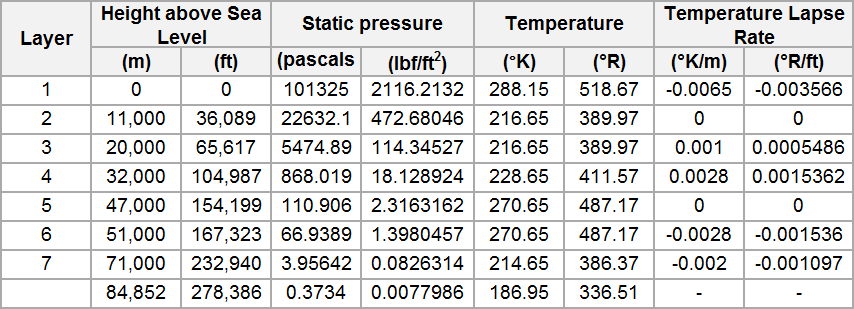
\includegraphics[width=0.9\textwidth]{atmostable.png}
\caption{The atmospheric table listing U.S. Standard Atmosphere properties}
\label{fig:Figure0}
\end{figure}

\begin{figure}[here]
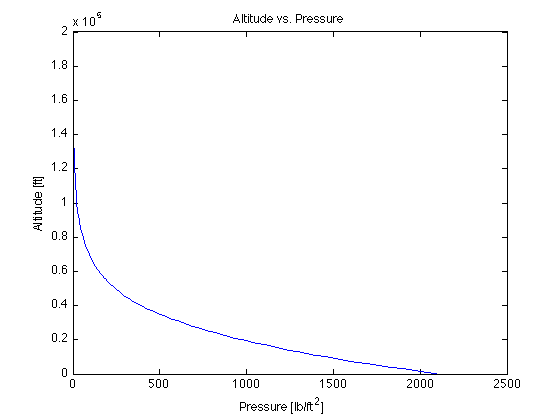
\includegraphics[width=1\textwidth]{AltitudeVsPressure.png}
\caption{Altitude versus Pressure}
\label{fig:Figure1}
\end{figure}

\begin{figure}[here]
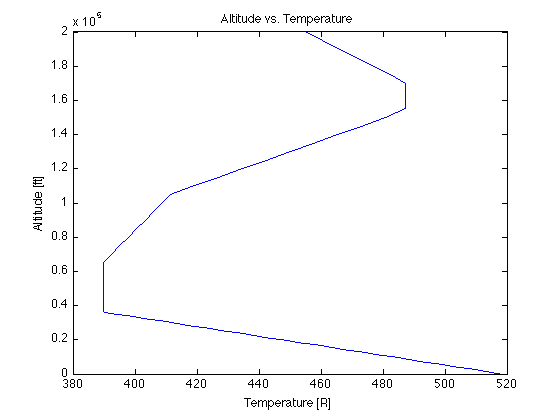
\includegraphics[width=1\textwidth]{AltitudeVsTemperature.png}
\caption{Altitude versus Temperature}
\label{fig:Figure2}
\end{figure}

\begin{figure}[here]
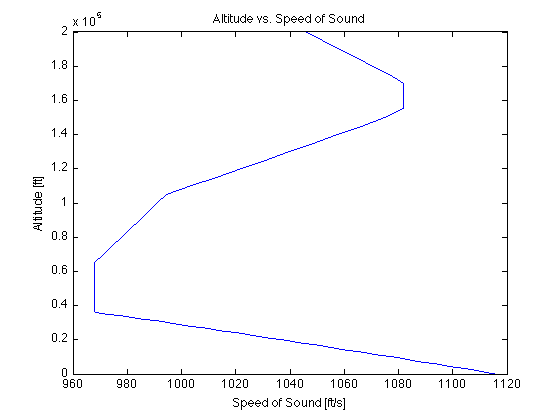
\includegraphics[width=1\textwidth]{AltitudeVsSpeedOfSound.png}
\caption{Altitude versus Speed Of Sound}
\label{fig:Figure3}
\end{figure}

\begin{figure}[here]
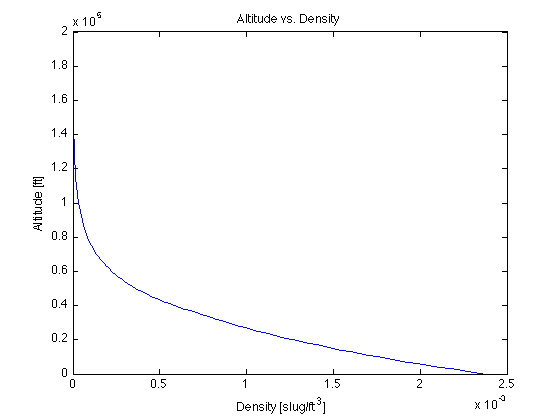
\includegraphics[width=1\textwidth]{AltitudeVsDensity.png}
\caption{Altitude versus Density}
\label{fig:Figure4}
\end{figure}

\begin{figure}[here]
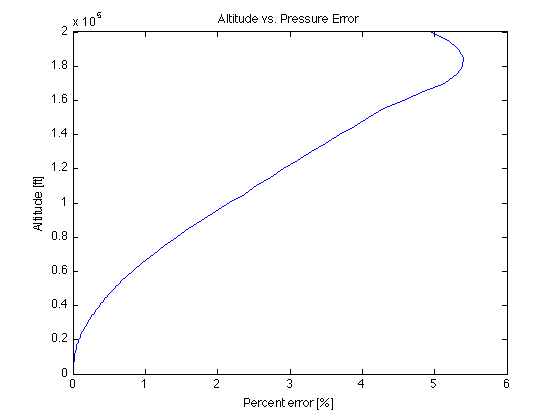
\includegraphics[width=1\textwidth]{AltitudeVsPressureError.png}
\caption{Altitude versus Pressure Error}
\label{fig:Figure5}
\end{figure}

\begin{figure}[here]
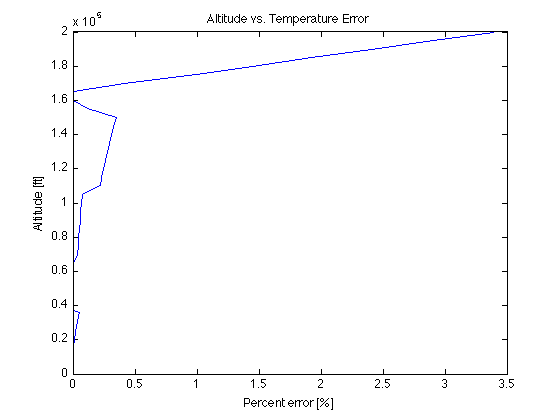
\includegraphics[width=1\textwidth]{AltitudeVsTemperatureError.png}
\caption{Altitude versus Temperature Error}
\label{fig:Figure6}
\end{figure}

\begin{figure}[here]
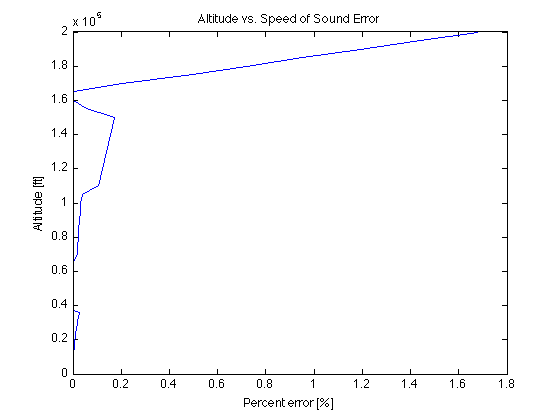
\includegraphics[width=1\textwidth]{AltitudeVsSpeedOfSoundError.png}
\caption{Altitude versus Speed Of Sound Error}
\label{fig:Figure7}
\end{figure}

\begin{figure}[here]
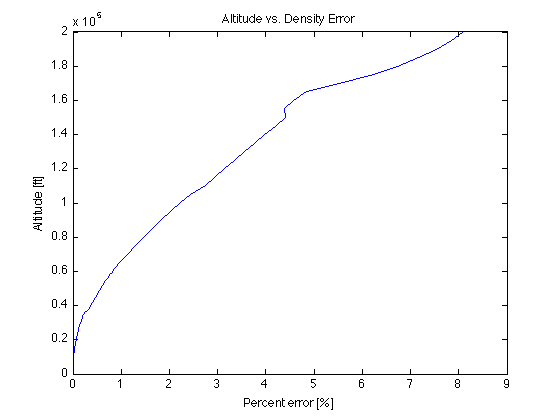
\includegraphics[width=1\textwidth]{AltitudeVsDensityError.png}
\caption{Altitude versus Density Error}
\label{fig:Figure8}
\end{figure}

\end{document}